\sloppy
\section{1. Кластер и программа расчета}

Работа выполнена 20 ноября 2026 года на macOS с процессором ARM64 и Docker
Desktop. В Docker доступны 12 CPU и 8 ГБ памяти. Через kind 0.27.0 поднят
Kubernetes 1.32.2 с узлом управления и рабочим узлом. Версия клиента kubectl
также 1.32.2. Рабочий kubelet резервирует 10 CPU через kube-reserved, поэтому
для планирования приложений остаются 2 CPU. Это заданное ограничение
учебного стенда. Оба узла находятся на одном компьютере.

Вариант 9, программист, разработчик на мобильных платформах. Из третьей
работы перенесены условие отбора вакансий, нормализация навыков, чтение S3
через GET Range и обработка границ строк. Образ lab5-pairs:1 собран из
python:3.12.12-slim-bookworm и содержит Python с boto3. Программа считает
только пары. Роль вакансии должна быть Программист, разработчик, а название
должно содержать мобильную платформу. Навыки приводятся к нижнему регистру,
повторы внутри вакансии удаляются. Каждая неупорядоченная пара учитывается
один раз на вакансию. Условию соответствуют 3771 вакансия.

Образ собран командой docker build с отключенными аттестациями provenance
и загружен в узлы kind. Dockerfile, программа и манифесты находятся в папке
работы. Ключи S3 передаются через Secret и не входят в образ.

\begin{figure}[H]
\centering
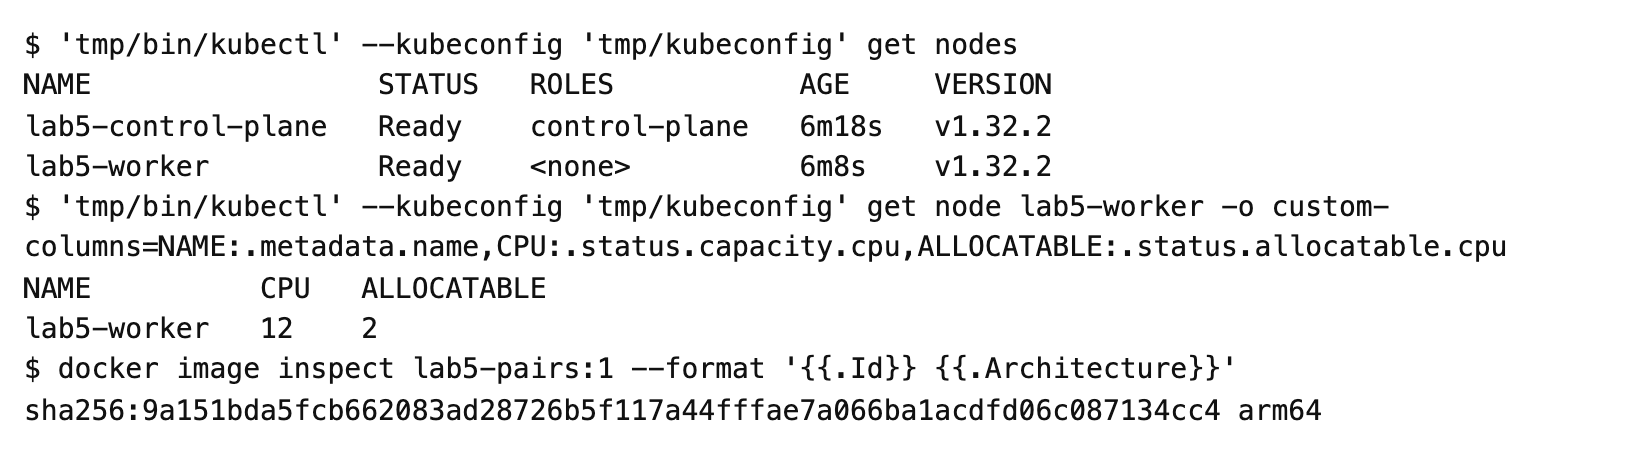
\includegraphics[width=\textwidth]{../screenshots/01_cluster.png}
\caption{Узлы Kubernetes, доступный CPU и идентификатор образа}
\end{figure}

Снимки далее показывают сохраненные выводы команд, открытые в браузере.
Полные журналы и JSON состояния Kubernetes сохранены в logs.

\newpage
\section{2. Остановка по памяти и выбор предела}

Первый Job pairs-oom читает исходный объект из внешнего RustFS через
host.docker.internal на порту 9010. Заявка CPU равна 500m, предел CPU равен
1, заявка и предел памяти равны 64 МиБ. Установлены restartPolicy Never и
backoffLimit 0, поэтому неуспешная попытка сохраняется для проверки.
Контейнер действительно остановлен с причиной OOMKilled и кодом 137.
Это остановка процесса при превышении памяти, а не ошибка чтения S3.

Следующий Job pairs-measure выполняет тот же расчет с пределом 512 МиБ.
Пик памяти процесса получен через getrusage, пик всей группы контейнера
через memory.peak в cgroup v2. Пик RSS равен 119046144 байтам, пик cgroup
равен 112902144 байтам, или 107,67 МиБ. Эти показатели имеют разный учет
общих страниц и служебной памяти. Для лимита контейнера использован пик
cgroup. Он записан после вычисления и выгрузки основного результата.

К измеренному пику добавлен запас 25 процентов, результат округлен вверх
до кратного 32 МиБ. Расчет имеет вид
$L = 32\lceil 107{,}67 \cdot 1{,}25 / 32 \rceil = 160$ МиБ.
Job pairs-sized с пределом 160 МиБ успешно завершился. Его пик cgroup
равен 111972352 байтам, или 106,79 МиБ, время программы 7,446 секунды.
Полученный файл полностью совпал с третьей работой.

\begin{figure}[H]
\centering
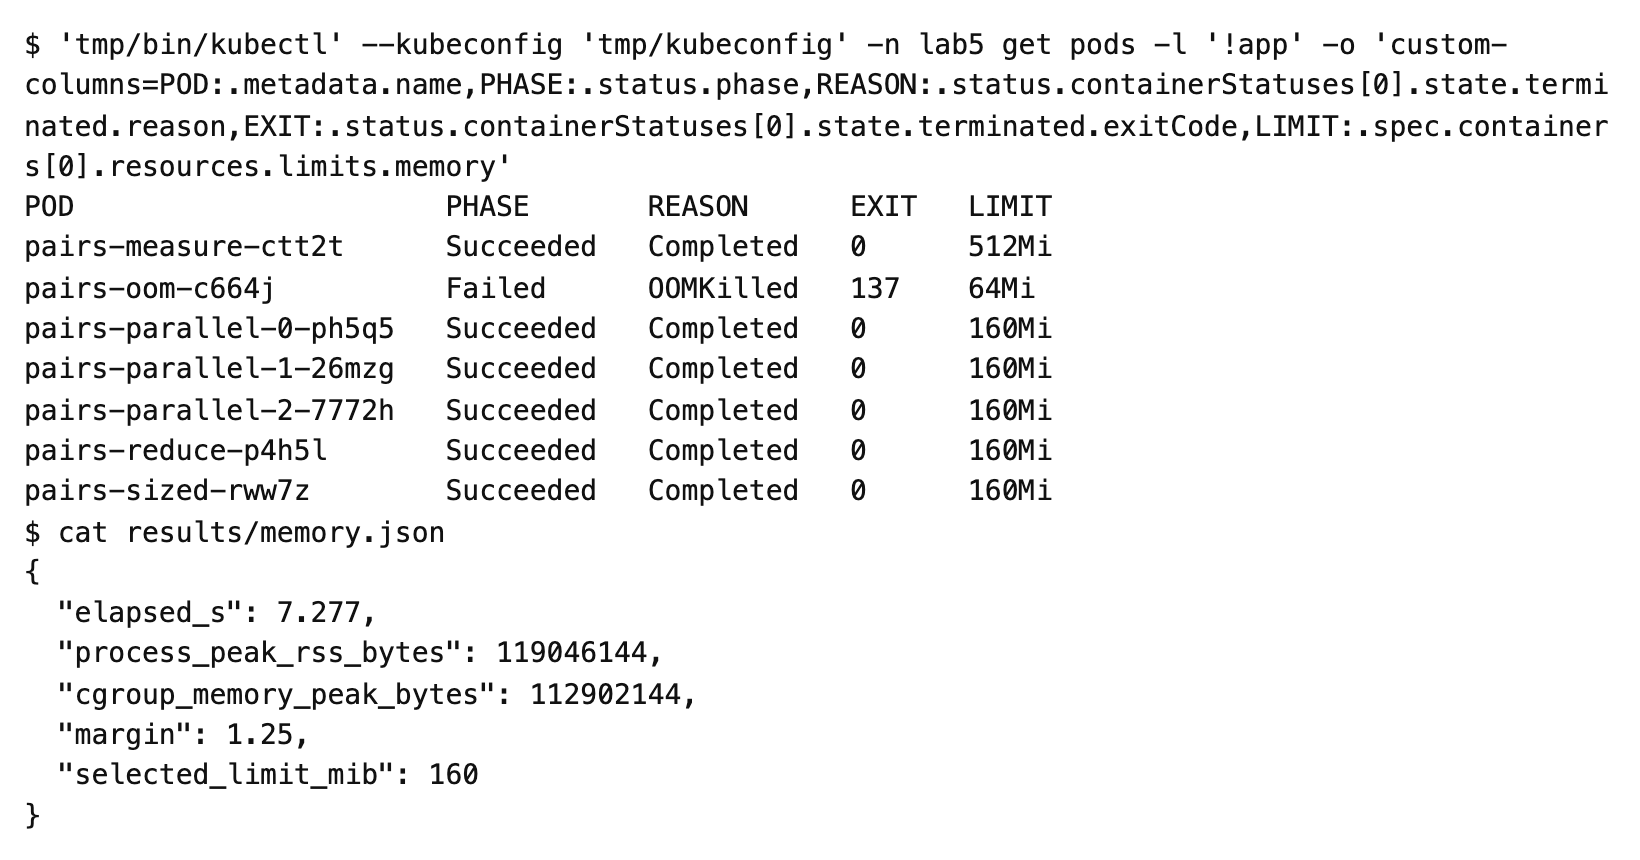
\includegraphics[width=\textwidth]{../screenshots/02_memory.png}
\caption{OOMKilled, успешные задания и измерение для выбора предела памяти}
\end{figure}

Request используется при планировании и не является верхней границей
потребления. Поэтому заявка памяти 64 МиБ не мешает успешному расчету с
пределом 160 МиБ. Превышение предела CPU приводит к ограничению времени
процессора, а превышение предела памяти может завершить контейнер.

\newpage
\section{3. Перенос RustFS в Kubernetes}

Хранилище RustFS 1.0.0 развернуто внутри кластера как Deployment с одной
репликой. Service rustfs предоставляет порт 9000, приложения обращаются
к нему по имени rustfs. PersistentVolumeClaim rustfs-data запрашивает
5 ГиБ. На томе находятся четыре папки vol1, vol2, vol3 и vol4. Сохранена
схема EC 2+2 из второй работы. Четыре папки на одном томе не дают защиты
от отказа самого компьютера.

Init-контейнер создает папки и назначает владельца с UID 10001, под которым
работает RustFS. Само хранилище запрашивает 250m CPU и 256 МиБ памяти,
пределы равны 1 CPU и 2 ГиБ. Ему назначен приоритет 2000, чтобы проверка
вытеснения вычислений не остановила хранилище.

Входной объект из бакета hh-lake третьей работы перенесен через S3 API в
бакет с тем же именем внутри кластера. Размер CSV равен 847619384 байтам.
Контрольные суммы SHA256 исходного объекта и объекта после переноса
совпали. Port-forward используется только для переноса и проверки с
компьютера. Вычислительные Pod читают данные непосредственно через Service
внутри Kubernetes.

\begin{figure}[H]
\centering
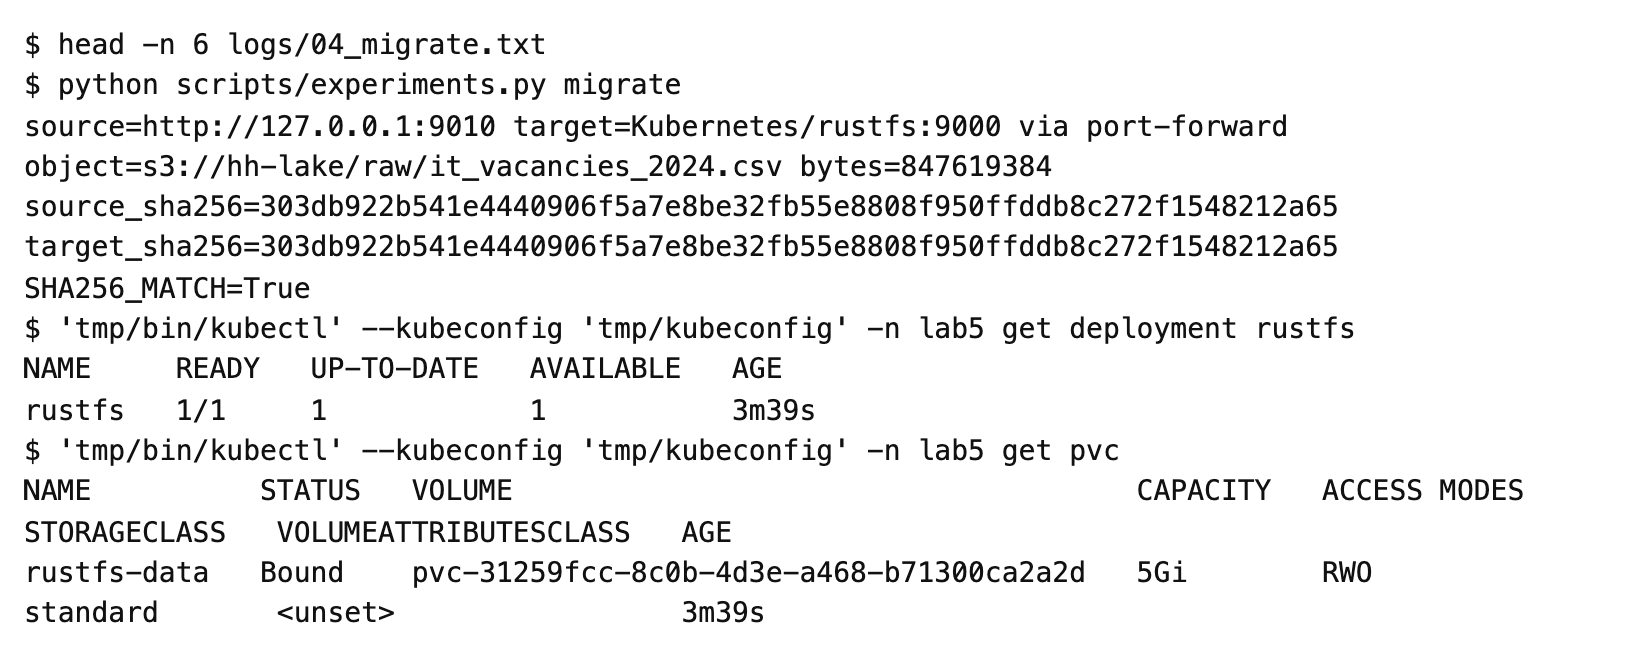
\includegraphics[width=\textwidth]{../screenshots/03_storage.png}
\caption{Перенос CSV с проверкой SHA256 и постоянный том RustFS}
\end{figure}

PVC связан с локальным томом внутри рабочего узла kind. Его данные
сохраняются при замене Pod хранилища, но удаление всего локального кластера
удалит и этот том. Исходное хранилище предыдущей работы сохранено.

\newpage
\section{4. Параллельный расчет по частям файла}

Использован Indexed Job pairs-parallel с тремя завершениями и
parallelism 3. Kubernetes передает каждому Pod индекс от 0 до 2 через
JOB\_COMPLETION\_INDEX. Объект делится на 26 сплитов по 32 МиБ, последний
сплит короче. Сплит с номером $i$ получает Pod с индексом $i \bmod 3$.
Поэтому два Pod обрабатывают по 9 сплитов, третий 8.

Строка принадлежит сплиту, в котором находится ее первый байт. Начало
неполной строки пропускается, последняя строка дочитывается за границей
сплита. Это сохраняет исходную обработку третьей работы. Каждый Pod
считает пары своих вакансий и записывает частичные частоты в S3 под своим
индексом. Повторная попытка использует то же имя объекта и не добавляет
еще одну копию частот.

Каждый Pod запрашивает 500m CPU и 64 МиБ памяти. Пределы равны 1 CPU и
160 МиБ. Суммарная заявка трех Pod равна 1500m, вместе с 250m RustFS она
укладывается в доступный CPU узла с учетом системных Pod. Все три
контейнера работали одновременно с 08:00:00 до 08:00:03 UTC. Пики их
cgroup составили 111,34, 109,68 и 109,08 МиБ, что ниже выбранного предела.

\begin{figure}[H]
\centering
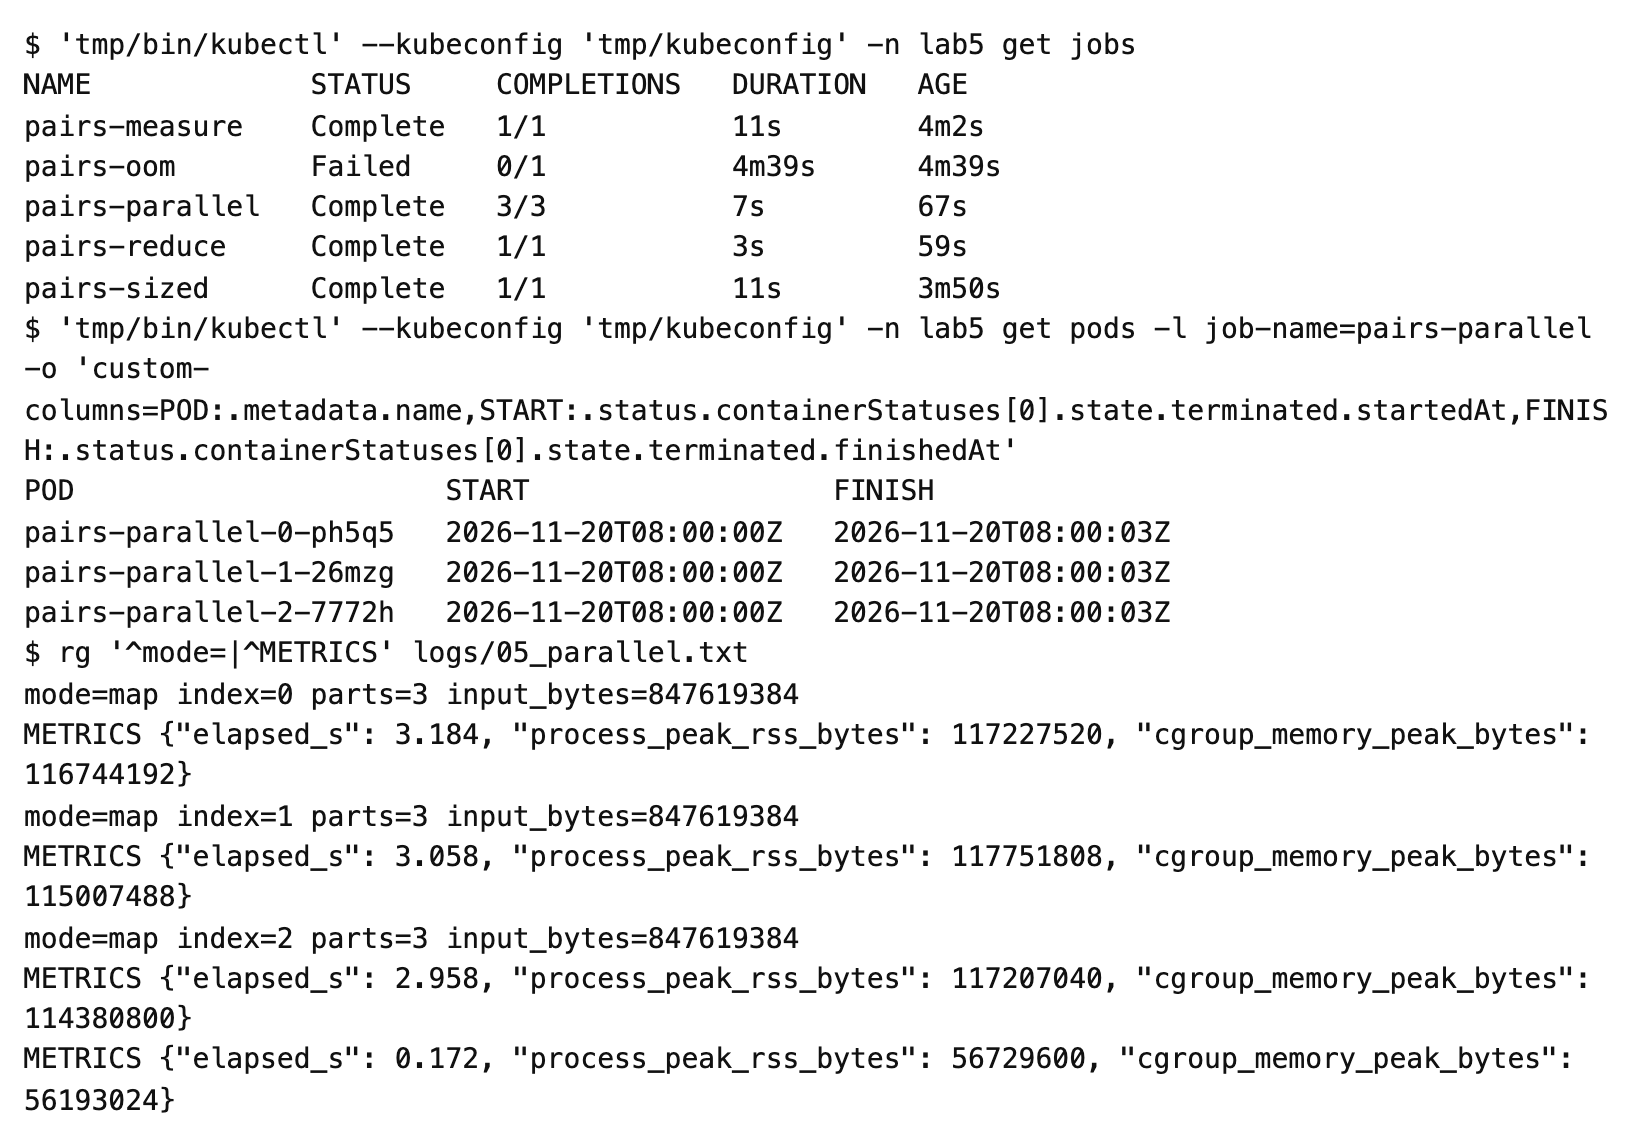
\includegraphics[width=\textwidth]{../screenshots/04_parallel.png}
\caption{Три завершенных Pod, пересекающееся время работы и потребление памяти}
\end{figure}

После успешного завершения всех трех частей запускается Job pairs-reduce.
Он читает три файла частот из S3, суммирует одинаковые пары и сортирует
результат по убыванию частоты, затем по названиям навыков. Итог сохраняется
в объект lab5/parallel/pairs.csv того же бакета.

\newpage
\section{5. Сверка с третьей работой}

В качестве эталона сохранен файл skills\_k2.csv третьей работы. Проверка
сравнивает все строки одиночного и параллельного результатов с эталоном,
включая порядок пар и частоты. В обоих результатах 12308 различных пар,
сумма частот 48175. Полные результаты совпали, значит совпал и топ-10.
В этом запуске совпали также байты CSV и SHA256.

Самая частая пара android и kotlin встречается в 784 вакансиях, ios и
swift в 561, android sdk и kotlin в 514. Все десять пар приведены в выводе
проверки. Файлы одиночного и параллельного результатов, эталон и отдельный
топ-10 сохранены вместе с программой проверки.

\begin{figure}[H]
\centering
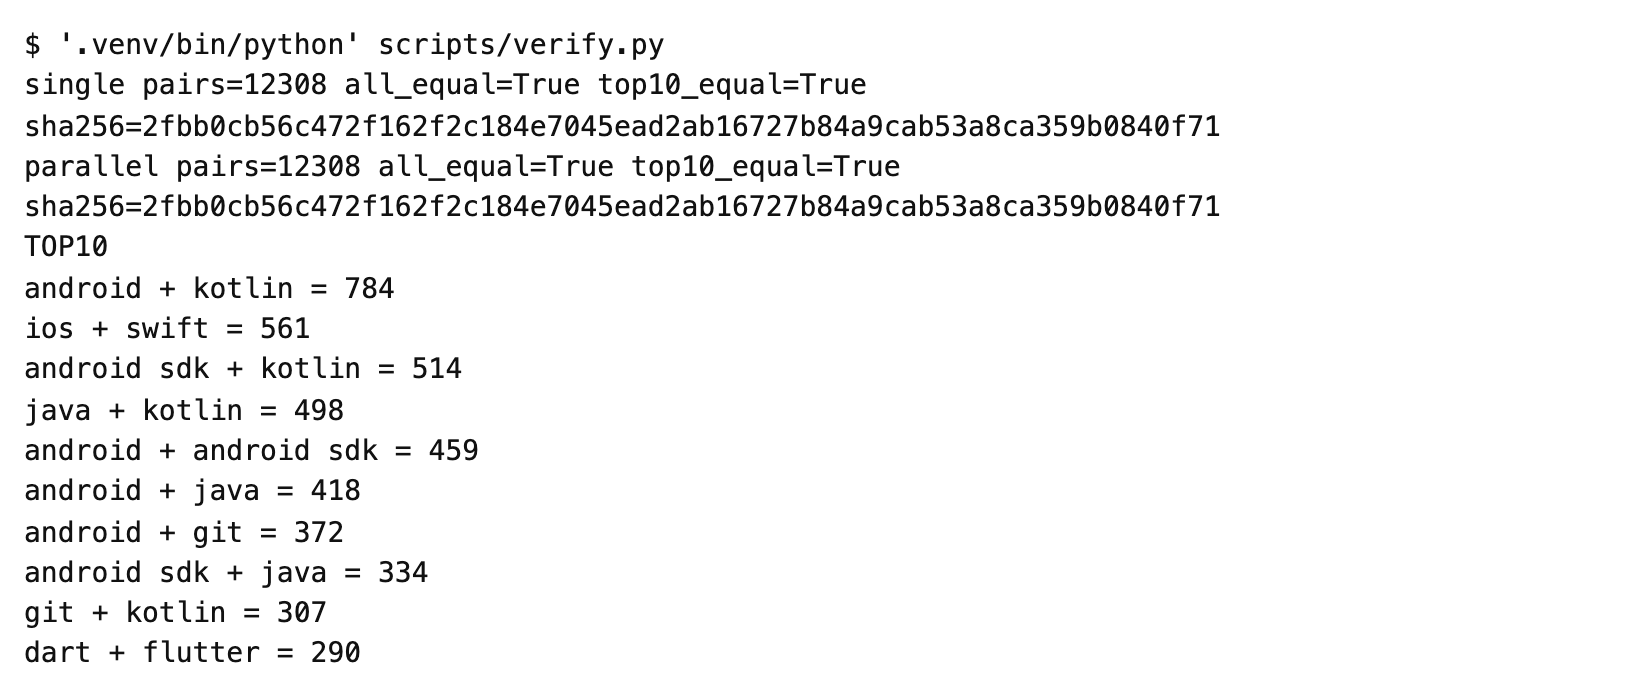
\includegraphics[width=\textwidth]{../screenshots/05_verify.png}
\caption{Полное совпадение результатов и итоговые десять пар навыков}
\end{figure}

\newpage
\section{6. Ожидание свободного процессора}

Для отдельной проверки планирования запущен Pod cpu-holder с заявкой
1200m CPU. Затем создан cpu-wait с заявкой 1 CPU. Вместе с хранилищем
заявки составили 2450m, что больше доступных 2000m еще до учета системных
Pod. Cpu-wait остался Pending. В событии FailedScheduling указана причина
Insufficient cpu. Узел управления не рассматривается для расчета из-за
его taint, а все тестовые Pod направлены на рабочий узел.

Тестовые контейнеры выполняют ожидающий процесс. Это показывает, что
планировщик учитывает заявки, даже если процесс фактически почти не
загружает CPU. После удаления cpu-holder ожидающий Pod получил узел и
перешел в Running. В журнале сохранены оба состояния.

\begin{figure}[H]
\centering
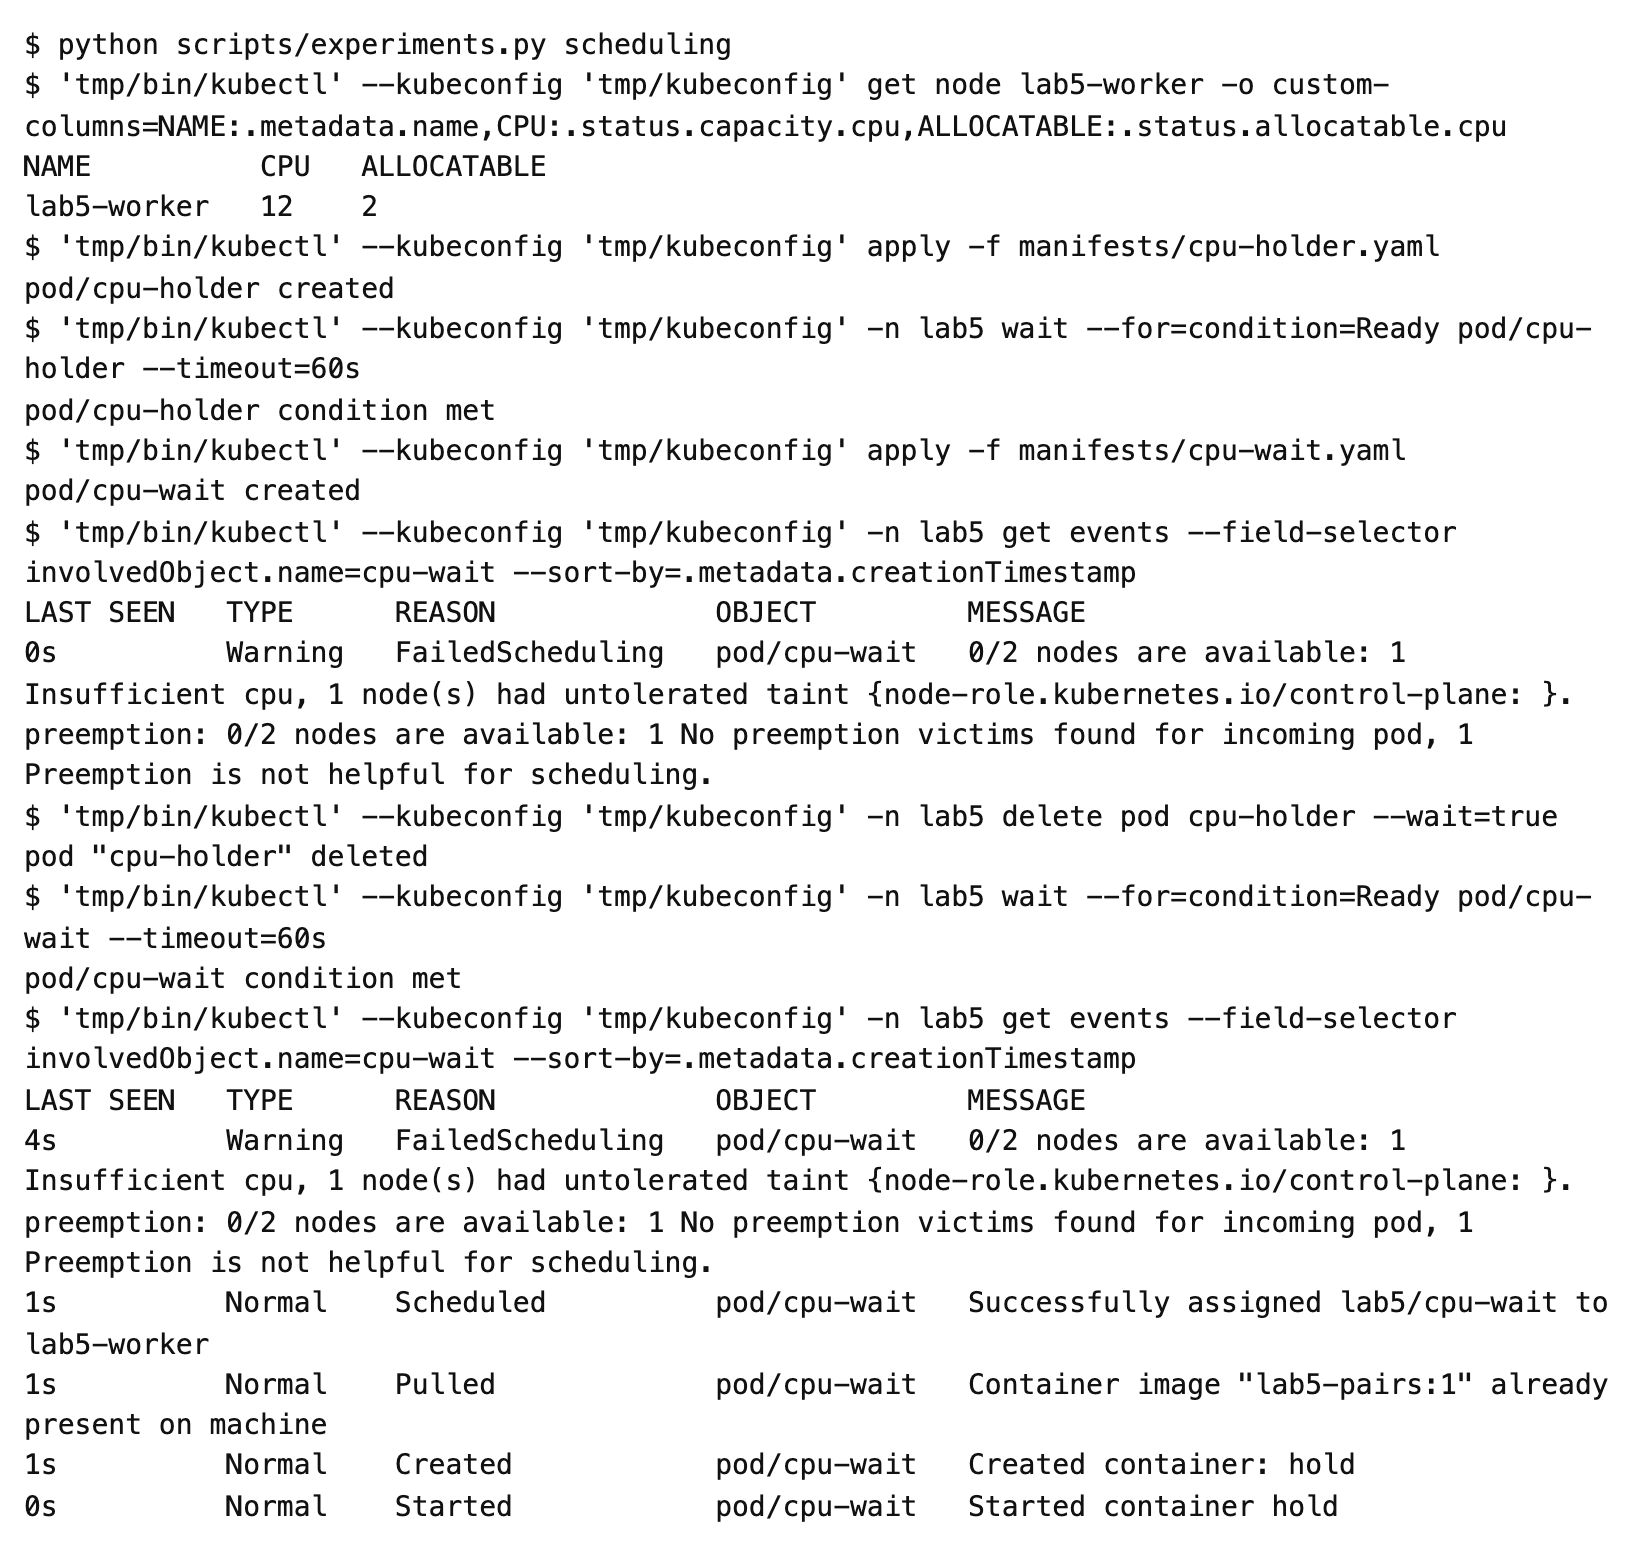
\includegraphics[width=\textwidth,height=0.78\textheight,keepaspectratio]{../screenshots/06_pending_1.png}
\caption{Нехватка CPU и запуск после освобождения заявки}
\end{figure}

\newpage
\section{7. Вытеснение по приоритету}

Созданы PriorityClass lab5-low со значением 10 и lab5-high со значением
1000. Оба разрешают PreemptLowerPriority. Низкоприоритетный Pod low
сначала получил 1200m CPU и перешел в Running. После этого создан Pod high
с заявкой 1 CPU. Свободного CPU для него не хватило.

Планировщик выбрал low жертвой вытеснения. В журнале есть событие Preempted
с идентификатором Pod high, затем Killing для low. После освобождения
ресурсов high получил рабочий узел и перешел в Running. Low удален.
Хранилище с приоритетом 2000 продолжило работу.

\begin{figure}[H]
\centering
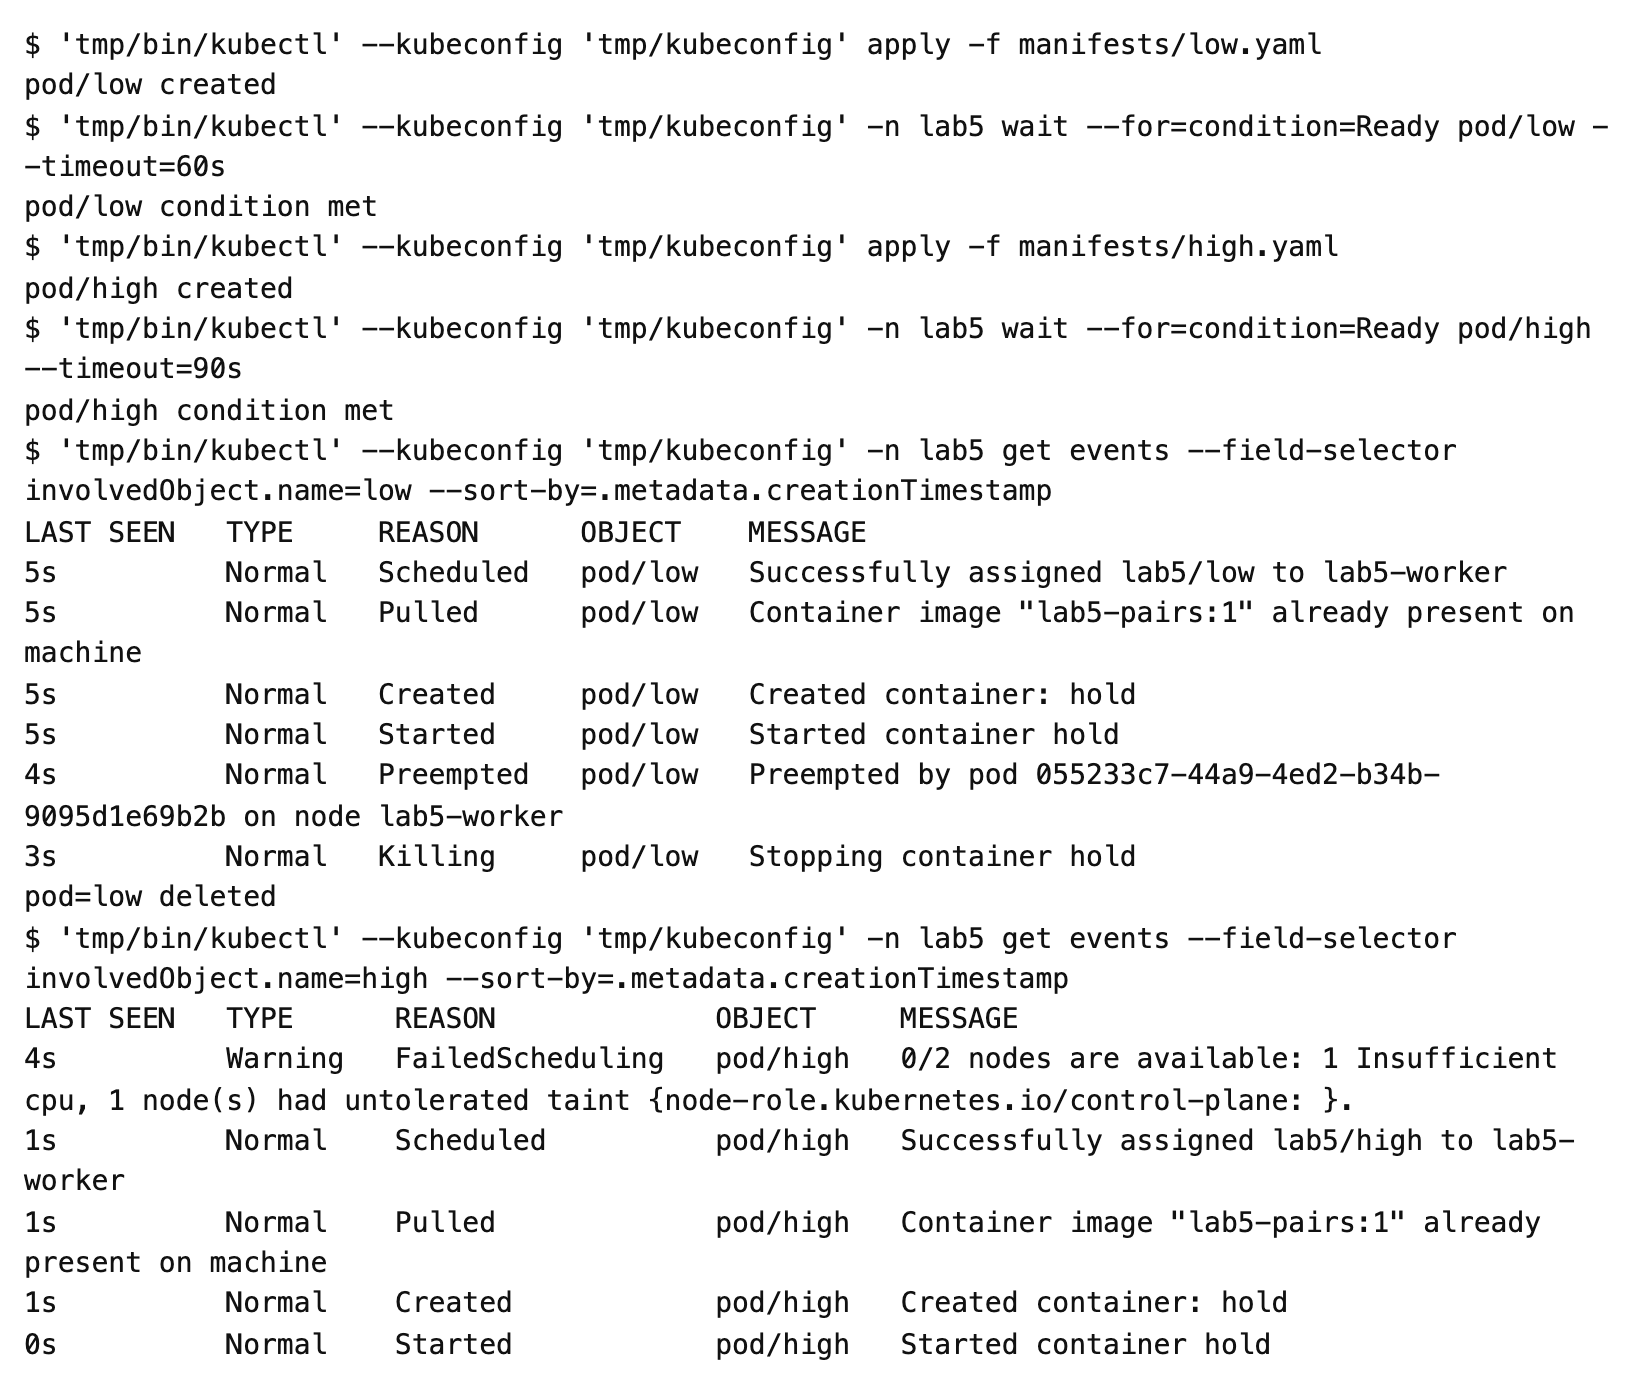
\includegraphics[width=\textwidth,height=0.78\textheight,keepaspectratio]{../screenshots/07_preemption_1.png}
\caption{Вытеснение low и запуск high по решению планировщика}
\end{figure}

Высокий приоритет не создает дополнительные ресурсы. Он позволяет
освободить их за счет Pod с меньшим приоритетом, если после этого задача
сможет разместиться. Непомещающаяся даже на свободный узел задача осталась
бы в ожидании. В этом опыте вытеснение вызвано заявками CPU, а не OOM.

\newpage
\section{8. Квота пространства имен}

В отдельном namespace lab5-quota создана ResourceQuota compute. Суммарная
заявка CPU ограничена 600m, заявка памяти 128 МиБ, предел CPU 1, предел
памяти 256 МиБ, количество активных Pod ограничено двумя.

Первый Pod quota-first запрашивает 400m CPU и 32 МиБ памяти. Он успешно
создан и запущен. Второй Pod quota-second с такой же заявкой требует
суммарно 800m CPU. API отклонил его создание с Forbidden и exceeded quota.
В сообщении указаны requested 400m, used 400m и limited 600m.

\begin{figure}[H]
\centering
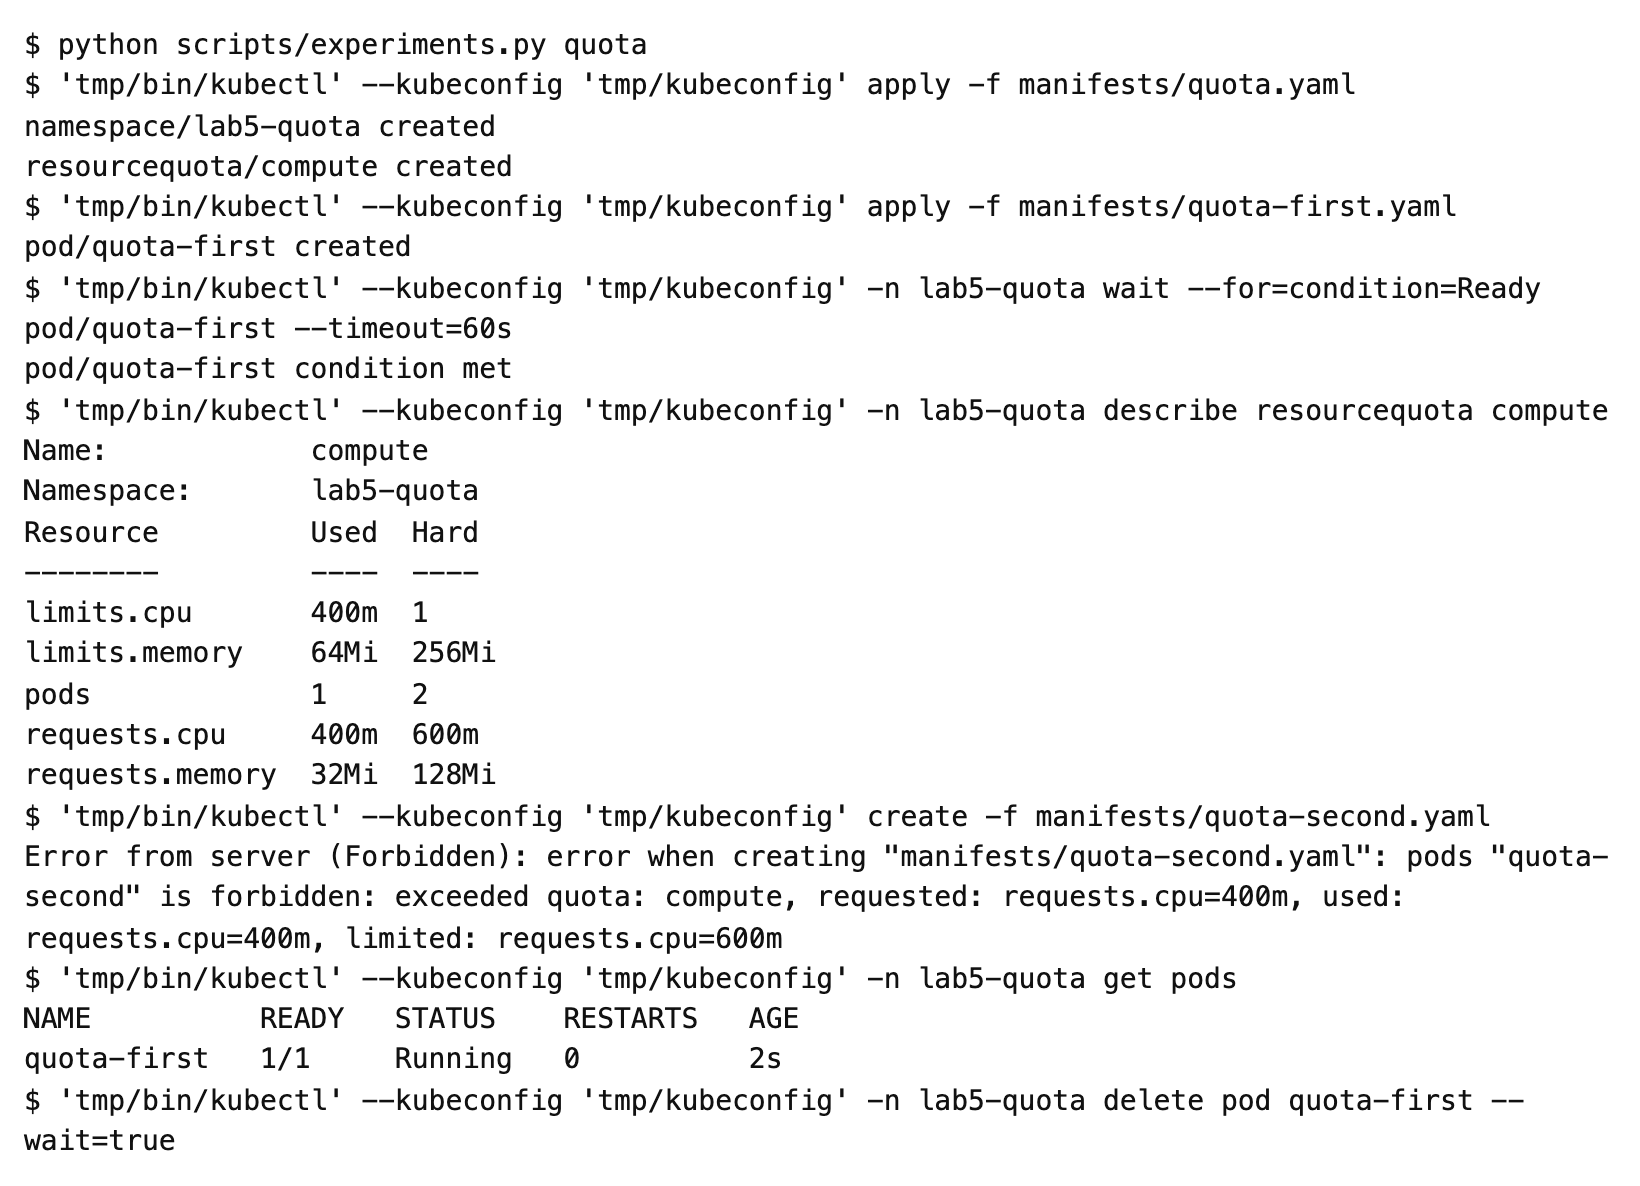
\includegraphics[width=\textwidth,height=0.72\textheight,keepaspectratio]{../screenshots/08_quota_1.png}
\caption{Использование квоты и отказ в создании второго Pod}
\end{figure}

После удаления quota-first тот же манифест quota-second успешно принят,
Pod перешел в Running. Следовательно, отказ связан с суммой заявок в
namespace, а не с образом или конфигурацией контейнера.

Квота проверяется при приеме объекта через API. Это отличается от
FailedScheduling, когда Pod уже создан, но планировщик не может найти ему
узел. При превышении квоты второго Pod вообще не было в списке объектов.

\newpage
\section{9. Соответствие YARN, Mesos и Kubernetes}

\subsection{Кто распределяет ресурсы и запускает задачи}

В YARN ResourceManager управляет ресурсами кластера, Scheduler распределяет
контейнеры, NodeManager запускает их на узле. ApplicationMaster относится
к конкретному приложению, запрашивает контейнеры и координирует расчет.

В Kubernetes API server принимает объекты, scheduler выбирает узел для
Pod, kubelet запускает контейнеры через среду исполнения. Контроллер Job
следит за завершениями и повторными попытками. Полного аналога
ApplicationMaster нет. У нас контроллер запускает три Pod, программа
распределяет сплиты по индексам, а скрипт запускает reduce после map.

В Mesos master предлагает ресурсы фреймворкам, agent управляет исполнением
на узле. Фреймворк имеет собственный scheduler и executors. Scheduler
выбирает задачи для предложенных ресурсов, executor выполняет их.
Роль agent близка к NodeManager и kubelet, но их интерфейсы различаются.

\subsection{Как различаются модели планирования}

YARN принимает запросы приложений, глобальный Scheduler распределяет
контейнеры с учетом очередей. ApplicationMaster отвечает за задачи
приложения. Kubernetes также централизованно выбирает узел для Pod
по requests, ограничениям размещения и приоритетам.

В Mesos планирование двухуровневое. Master предлагает ресурсы конкретных
узлов, scheduler фреймворка принимает или отклоняет предложение и выбирает
задачи. Отклоненные ресурсы могут получить другие фреймворки. В наших Job
Kubernetes такого обмена предложениями нет, узел выбирает scheduler.

\subsection{Как соотносятся очереди, приоритеты и квоты}

FIFO обслуживает заявки по порядку, поэтому короткая задача может ждать
за большой. Capacity Scheduler в YARN задает доли очередей, допускает
использование свободной емкости и вытеснение. Fair Scheduler стремится
справедливо делить ресурсы. В Mesos политика распределения определяет,
кому предлагать ресурсы, а фреймворк выбирает задачи.

В Kubernetes requests нужны для планирования, limits ограничивают
исполнение, PriorityClass влияет на порядок и вытеснение, ResourceQuota
ограничивает сумму ресурсов namespace. Квота не гарантирует долю CPU,
не резервирует ресурсы заранее и сама не обеспечивает справедливость.
В опытах получены Pending, Preempted и отказ API по квоте.

\section{Вывод}

Предел 160 МиБ выбран по измеренному пику и проверен успешным запуском.
Все сценарии ресурсов выполнены, параллельный расчет из S3 внутри кластера
совпал с третьей работой по всем парам и топ-10.

\href{https://github.com/Gegerout/data-engineering-lab5}{Репозиторий работы с кодом, манифестами и журналами.}

\section{Источники}

\href{https://kubernetes.io/docs/concepts/configuration/manage-resources-containers/}{Документация Kubernetes по ресурсам контейнеров.}
\href{https://kubernetes.io/docs/concepts/scheduling-eviction/pod-priority-preemption/}{Приоритеты и вытеснение Kubernetes.}
\href{https://kubernetes.io/docs/concepts/policy/resource-quotas/}{Квоты Kubernetes.}
\href{https://hadoop.apache.org/docs/stable/hadoop-yarn/hadoop-yarn-site/YARN.html}{Архитектура Apache Hadoop YARN.}
\href{https://mesos.apache.org/documentation/latest/architecture/}{Архитектура Apache Mesos.}
